\documentclass[10pt]{beamer}
\usepackage[latin1]{inputenc}
%\documentclass{article}
\usepackage{graphicx}
\usepackage[T1]{fontenc}
\usepackage[english]{babel}
\usepackage{multimedia}
\usepackage{graphicx,dsfont,color,subfigure}
\usepackage{amsmath,graphicx,dsfont,color}
\usepackage{amsfonts}
\usepackage{amssymb}

% Example definitions.
% --------------------
\def\x{{\mathbf {x}}}
\def\realset{{\mathbb{R}}}
\def\dimension{D}
\def\thr{\tau}
\def\mean{\text{mean}}
\def\std{\text{st.dev.}}
 \newcommand{\anomaly}[1]{\mathcal{D}(#1)}
 \newcommand{\vectorI}{\x}
 \newcommand{\median}{\text{MED}}
\newcommand{\mad}{\text{MAD}}
\newcommand{\SSigma}{\boldsymbol\Sigma}
\newcommand{\mmu}{\boldsymbol{\mu}}
\newcommand{\matrixI}{\mathbf{X}}
\newcommand{\vectorZ}{\vectorB}
\newcommand{\vectorB}{\mathbf{b}}
\newcommand{\proj}{\mathbf{u}}
\newcommand{\Proj}{\mathbf{U}}
\newcommand{\nr}{n_1}
\newcommand{\nc}{n_2}
\newcommand{\nb}{n_3}
\newcommand{\nscales}{m}
\newcommand{\nsize}{n}
\newcommand{\iterindex}{i}
\newcommand{\rep}{r}
\newcommand{\depth}[2]{PD(#1;#2)}
\newcommand{\MED}{\text{MED}}
\newcommand{\MAD}{\text{MAD}}
\newcommand{\mmux}{\mmu_{\matrixI}}
\newcommand{\Sigmax}{\SSigma_{\matrixI}}


\mode<presentation> {
    %\usetheme{JuanLesPins}
    \usetheme{Montpellier}
    \setbeamertemplate{footline}[frame number]%pour ajouter le num?ro de page
    \setbeamertemplate{footline}[text line]{S. Velasco-Forero. velasco@cmm.ensmp.fr. \'Ecole des Mines de Paris. MINES-PARISTECH}
    \setbeamertemplate{navigation symbols}{}%Pour enlever la barre de navigation
    \setbeamertemplate{blocks}[rounded][shadow=true] 
}

\title{Anomaly Detection}
\author{Santiago Velasco-Forero\\
\texttt{\scriptsize santiago.velasco@mines-paristech.fr} ; \texttt{\scriptsize http://cmm.ensmp.fr/$\sim$velasco}\\ %\bigskip
}

\institute{\emph{CMM-Centre de Morphologie Math\'{e}matique,}
Math\'{e}matiques et Syst\`{e}mes, MINES-PARISTECH, FRANCE }


\date{\alert{Deep Learning Course 2020}}

\def\newblock{\hskip .11em plus .33em minus .07 em}
\begin{document}

%\begin{frame}
%\titlepage
%\end{frame}

%===============================================================================
\begin{frame}
    \titlepage
%     \begin{columns}
%        \begin{column}[l]{6cm}
%            \begin{figure}
%                \includegraphics[width=0.2\columnwidth]{./figures/logo-emp-b.png}
%            \end{figure}
%        \end{column}
%        \begin{column}[r]{6cm}
%            \begin{figure}
%                \includegraphics[width=0.5\columnwidth]{./figures/CMM-logo.png}
%            \end{figure}
%        \end{column}
%    \end{columns}
\end{frame}
%===============================================================================



\begin{frame}
    \frametitle{Plan}
    %\tableofcontents[hideallsubsections]%[pausesections]
    \tableofcontents%[pausesections]
\end{frame}

%\section{Introduction}

%\begin{frame}
%A common need when analyzing real-world data-sets is determining which instances stand out as being dissimilar
%to all others. Such instances are known as \alert{anomalies}, and the goal of anomaly detection (also known as \alert{outlier
%detection}) 
%How can we look for something when we don't know what are we looking for?\\
%
%Outlier is defined as an observation that deviates too
%much from other observations that it arouses suspicions that
%it was generated by a different mechanism from other observations. (
%The exact definition of an outlier depends on the contex)
%\end{frame}
%
%\begin{frame}
%\onslide <2-> \centering{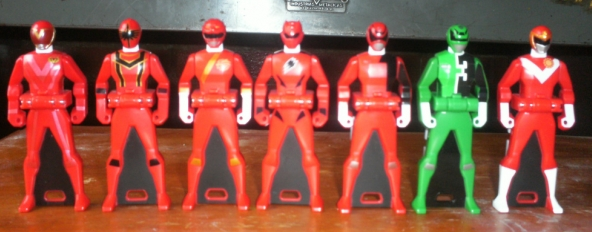
\includegraphics[width=.4\columnwidth]{Mistake2}}\\
%\onslide <3->\centering{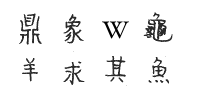
\includegraphics[width=.4\columnwidth]{Letters}}
%\onslide <4->\centering{
\includegraphics[width=.4\columnwidth]{MarcasAutos}}
%\end{frame}


%\begin{frame}{Anomaly or novelty?}
%Problem 1:
%\begin{center}
% 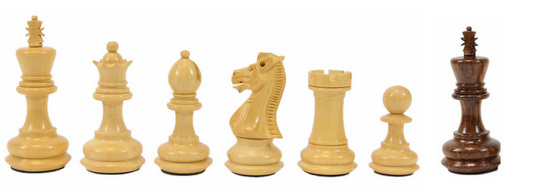
\includegraphics[width=.5\columnwidth]{Anomaly1}
%\end{center}\pause
%Problem 2:
%\begin{center}
% 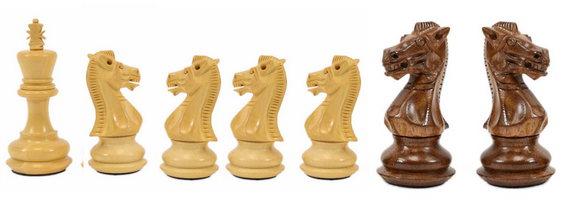
\includegraphics[width=.5\columnwidth]{Anomaly3}
%\end{center}\pause
%\end{frame}
%
%\begin{frame}{Novelty or Anomaly}
%Novelty detection is the identification of a novel (new) or unobserved patterns in the data. For instance, in Figure the images of (white tigers) among regular tigers may be considered as a novelty, while the image of (horse, panther, lion, and cheetah) are considered as anomalies. The techniques used for anomaly detection are often used for novelty detection and vice versa.
%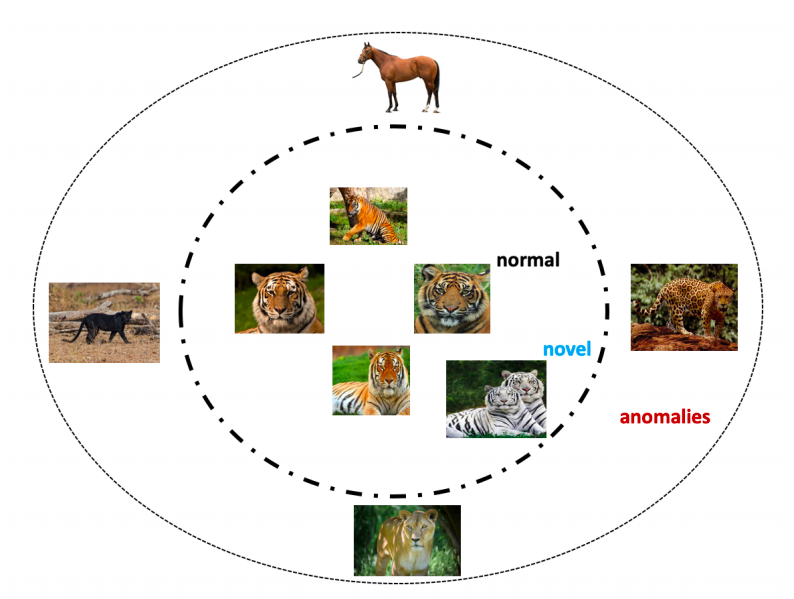
\includegraphics[width=.8\columnwidth]{Novelty}
%\end{frame}

\section{Taxonomy}
\begin{frame}{Taxonomy}
\begin{center}
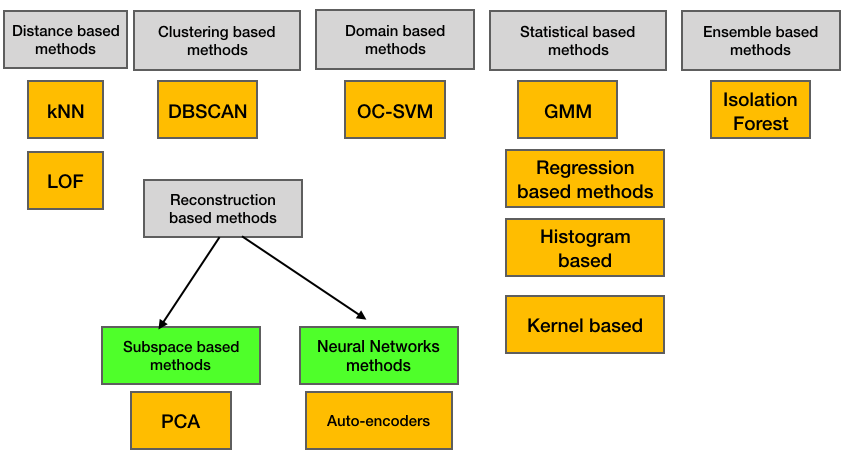
\includegraphics[width=.95\columnwidth]{TaxonomyOutliers}
\end{center}
\end{frame}


\section{Distance based methods}

\begin{frame}{kNN distance for outlier detection}
\begin{center}
 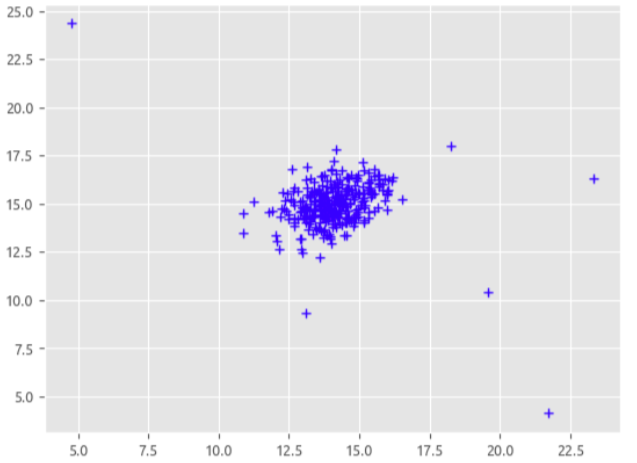
\includegraphics[width=.45\columnwidth]{GaussianBi}
\end{center}
For an observation $\vectorI$ , its distance to its $k$th nearest neighbor could be viewed as the outlying score. It could be viewed as a way to measure the density.
Many kNN detectors are supported: 
\begin{enumerate}
\item largest: use the distance to the $k$th neighbor as the outlier score.
\item Mean k-NN: use the average of all $k$ neighbors as the outlier score.
\item Many variants...
\end{enumerate}
\end{frame}


\section{Statistical Modelling of anomaly detection}
\begin{frame}{Z-score Univariate Case}
\texttt{Z-score} is an important concept in statistics. \texttt{Z score} is also called standard score, the procedure is called \emph{standardization}. This score helps to understand if a data value is greater or smaller than mean and how far away it is from the mean. More specifically, \texttt{Z-score} tells how many standard deviations away a data point is from the mean.
For a given univariate samples $X=\{x_1,\ldots,x_\mathcal{N}\}$, the \texttt{Z score} is defined by
\begin{equation}
\texttt{Z-score}= \frac{x_i - \bar{x}}{\sigma}
\end{equation}
where $\sigma$ and  is the standard deviation and mean of the distribution of feature $x$, respectively, and $x_i$ is the value of the feature $x$ for the ith sample.
\begin{center}
 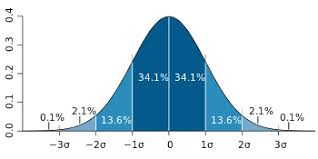
\includegraphics[width=.5\columnwidth]{zscore2}
\end{center}
\end{frame}

%\begin{frame}{Z-score for anomaly detection}
%\begin{center}
% 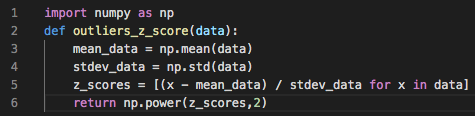
\includegraphics[width=.95\columnwidth]{ZscoreCode}
%\end{center}
%How can use this anomaly detector for multiple variables??
%\begin{center}
%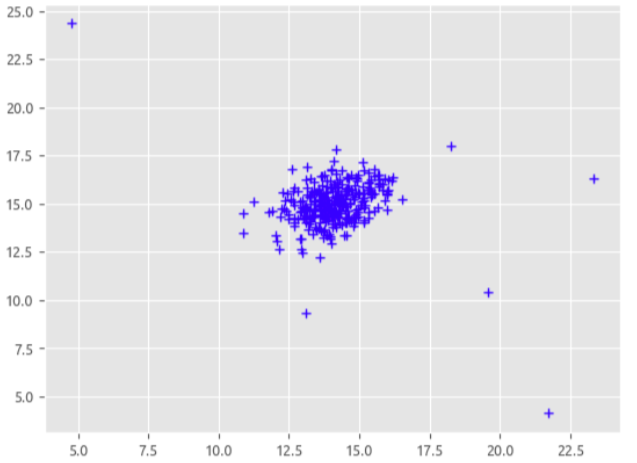
\includegraphics[width=.45\columnwidth]{GaussianBi}
%\end{center}
%\end{frame}

\begin{frame}{How to extend to multivariate case?}
 \begin{itemize}
\item  One approach to this problem would be to assume that the $\dimension$ variables are
 \emph{mutually independent}. 
 \item They may then be standardized so that,, each is normally distributed with zero mean and unit variance. \pause
 \item  Using sample estimates of the population parameters for the standarization, the sum of their squares is then asymptotically distributed like chi-square distribution.\pause
\item  \alert{In many application $p$ variables are not independent}. They are, in fact, very strongly correlated.
\end{itemize}
\end{frame}

\begin{frame}{Mahalanobis distance}
 This circumstance suggests the use of Hotelling's $T^2$ as the appropriate statistic. This statistics is computed by the \emph{sampled Mahalanobis distance}:
 \begin{equation}
M(\vectorI;\mmu,\SSigma)=(\vectorI - \mmu) \hat{\SSigma}^{-1} (\vectorI - \mmu)^T
\end{equation}
 where $\vectorI$ is the row vector whose elements are the observed values of the $\dimension$
 variables, $\mmu$ is the corresponding mean vector , and where $\hat{\SSigma}$ is the sample covariance matrix of the $\dimension$
 variables.
\begin{center}
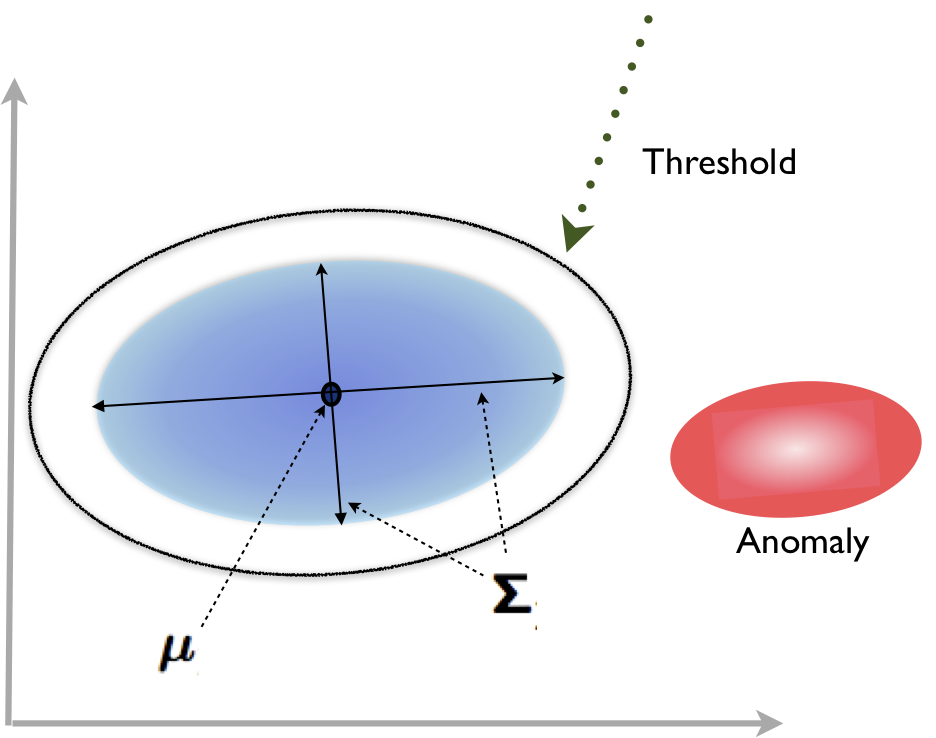
\includegraphics[width=.5\textwidth]{RXDetector}
\end{center}
\end{frame}

\begin{frame}{Covariance matrix estimation}
The sample covariance matrix of the observations $\vectorI_1,\ldots,\vectorI_\mathcal{N} \in \mathbb{R}^\dimension$ is defined by:
\begin{equation}
\hat{\SSigma}=\frac{1}{\mathcal{N} -1}\sum_{i=1}^{\mathcal{N} } (\vectorI_i-\bar{\vectorI})(\vectorI_i-\bar{\vectorI})^T
\end{equation}
Where, $\bar{\vectorI}$ denotes the empirical mean of the observations.
\end{frame}

\begin{frame}{Difficulties on high-dimensional spaces}
The use of this statistic gave rise to some difficulties. 
\begin{enumerate}
\item The determinant of the covariance matrix was found to be very small so that the computation of the inverse was inaccurate.
\item The smallness of the determinant of the covariance
 matrix indicated that the variates were so strongly correlated that some of them could be dropped from consideration.
 \item The estimation of  $\hat{\SSigma}$ depends of the relation between number of samples and the number of variables.
 \item Distance measures in high dimensional spaces has strange behaviours (Curse of Dimensionality).
 \item In general, intuition that we have in 3D are hard to extend to high dimensions.
 \end{enumerate}
 \end{frame}
 
 \begin{frame}{Curse of Dimensionality}
Connectivity in high dimensional spaces
$C^{\dimension}(\lambda)$ is the cube centered at the origin in $\realset^\dimension$ with side-length $2\lambda$
\begin{equation*}
C^{\dimension}(\lambda)=\{(x_1,\ldots,x_\dimension) | -\lambda \leq x_{j} \leq \lambda, \quad \forall j \}
\end{equation*}
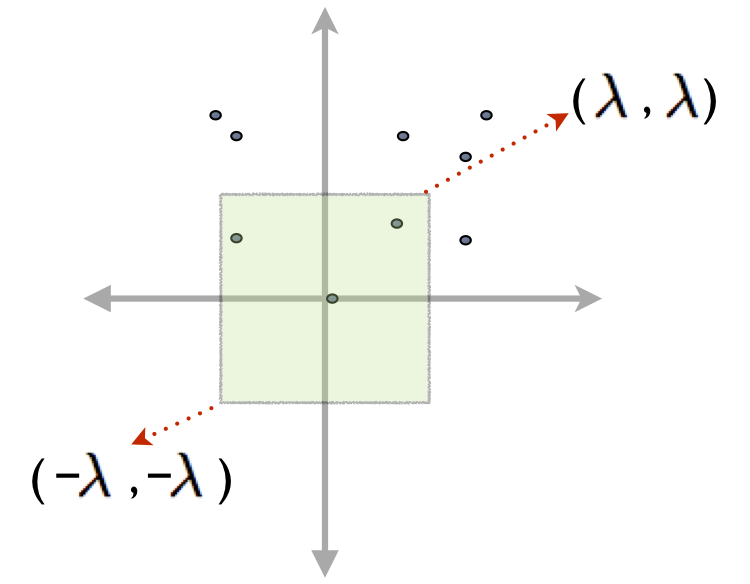
\includegraphics[width=.5\textwidth]{BoxLambda}
\alert{As $\dimension \to \infty$}, \textbf{Vol}$(C^{\dimension}(\lambda))=$
\end{frame}


\begin{frame}{Curse of Dimensionality}
\alert{As $\dimension \to \infty$}, \textbf{Vol} $(C^{\dimension}(\lambda))= (2\lambda \times 2\lambda \times \ldots \times 2\lambda)=(2\lambda)^{\dimension}$ \pause
\begin{eqnarray*}
\lim_{d \to \infty}\textbf{Vol}(C^{\dimension}(\lambda))= 0 \quad \text{if} \quad \lambda<1/2,\\ 
\lim_{d \to \infty}\textbf{Vol}(C^{\dimension}(\lambda))= \infty \quad  \text{if} \quad \lambda>1/2,\\ 
\lim_{d \to \infty}\textbf{Vol}(C^{\dimension}(\lambda))= 1 \quad \text{if} \quad \lambda=1/2
\end{eqnarray*}

\begin{eqnarray*}
\textbf{Diagonal} (C^{\dimension}(\lambda))=\pause 2\lambda\sqrt{\dimension}\\
\lambda=1/2 ,\text{ we obtain a cool shape!:} \\ \pause
\lim_{d \to \infty}\textbf{Vol}(C^{\dimension}(1/2))= 1 \\
\lim_{d \to \infty} \textbf{Diagonal}(C^{\dimension}(1/2))= \infty
\end{eqnarray*}
\end{frame}


%\begin{frame}
%\begin{columns}
%\begin{column}{.4 \textwidth}
%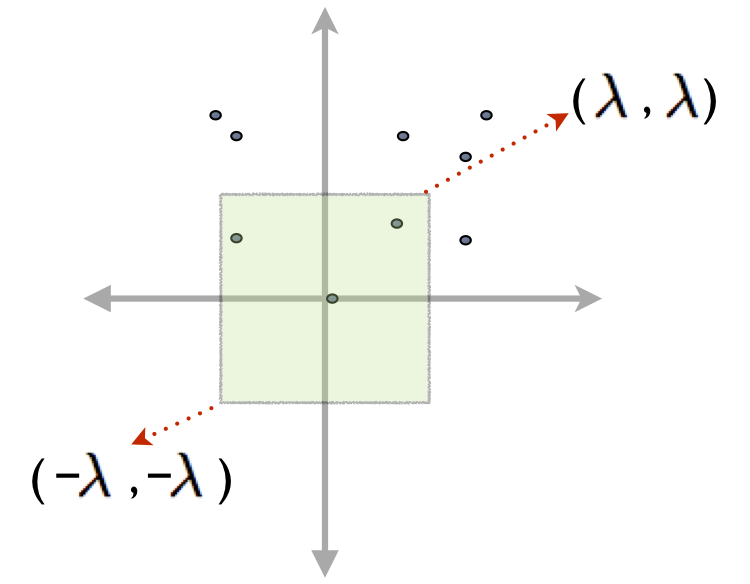
\includegraphics[width=1\textwidth]{BoxLambda}
%\end{column}
%\begin{column}{.6 \textwidth}
%\begin{eqnarray*}
%\lim_{d \to \infty}\textbf{Vol}(C^{\dimension}(\lambda))= 0 \quad \text{if} \quad \lambda<1/2,\\ 
%\lim_{d \to \infty}\textbf{Vol}(C^{\dimension}(\lambda))= \infty \quad  \text{if} \quad \lambda>1/2,\\ 
%\lim_{d \to \infty}\textbf{Vol}(C^{\dimension}(\lambda))= 1 \quad \text{if} \quad \lambda=1/2
%\end{eqnarray*}
%\begin{eqnarray*}
%\textbf{Diagonal} (C^{\dimension}(\lambda))=\pause 2\lambda\sqrt{\dimension}\\
%\lambda=1/2 ,\text{ we obtain:} \\ \pause
%\lim_{d \to \infty}\textbf{Vol}(C^{\dimension}(1/2))= 1 \\
%\lim_{d \to \infty} \textbf{Diagonal}(C^{\dimension}(1/2))= \infty
%\end{eqnarray*}
%\end{column}
%\end{columns}
%\end{frame}
 
 
 \begin{frame}{Using  subspaces}
 \begin{itemize}
\item  That is apply a linear dimensionality approach and then use a Mahalanobis distance or another method. 
\item (\alert{In this course}) A new set of $\dimension'$ variables ($\dimension'\leq \dimension$) is obtained by means of a linear transformation of the original variables. 
\item Since the transformation is linear  the multivariate normality of the new variables follows from that assumed for the original ones.
\item $y=(\vectorI-\mmu)\mathbf{W}$  where $\mathbf{W}$ is a $\dimension\times \dimension'$ rectangular matrix.
\begin{enumerate}
\item  Principal component analysis (PCA) : Columns are the properly normalized eigenvectors corresponding to the first $\dimension'$ largest eigenvalues of the
 sample covariance matrix $S$.
 \item  Negative Principal component analysis (NPCA) : Columns are the properly normalized eigenvectors corresponding to the first $\dimension'$ smallest eigenvalues of the
 sample covariance matrix $S$.
 \end{enumerate}
 \end{itemize}
 \end{frame}
 
\begin{frame}{Singular Value Decomposition}
The singular value decomposition of an $\dimension \times \mathcal{N} $ real or complex matrix $\mathbf {X}$ is a factorization of the form $\mathbf {U}\Lambda \mathbf{V}^{*}$, where $\mathbf {U}$ is an $\dimension\times \dimension$ real or complex unitary matrix, $\Sigma$ is an $m\times n$ rectangular diagonal matrix with non-negative real numbers on the diagonal, and $ \mathbf {V}$  is an  $\mathcal{N} \times \mathcal{N} $ real unitary matrix. If  $\mathbf {X}$ is real, $ \mathbf {U}$ and $ \mathbf {V}^{T} =\mathbf{V^{*}}$ are real orthogonal matrices. The diagonal entries $ \lambda_{i}=\Lambda_{ii}$ of  $\Lambda$ are known as the singular values of $\mathbf {X}$.
From the decomposition:
\begin{equation}
\mathbf{X}=\mathbf {U}\Lambda \mathbf{V}^{T} ,
\mathbf{X}^T\mathbf{X}=\mathbf{V} \Lambda^2 \mathbf{V}^T
\end{equation}
where $\Lambda$ contains the positive real eigenvalues of decreasing magnitude and the $i$-th eigenvalue equals the square of the $i$-th singular value
\end{frame} 

 


%\begin{frame}{Multiple Anomalies}
%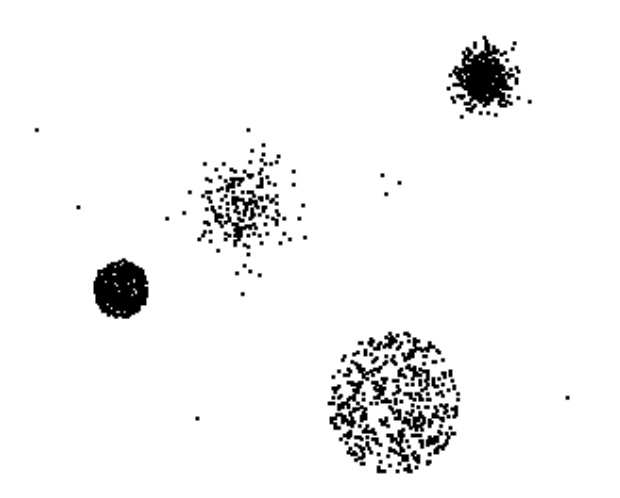
\includegraphics[width=.5\textwidth]{MultipleAnomalies}
%\end{frame}



\begin{frame}{Why local outliers?}
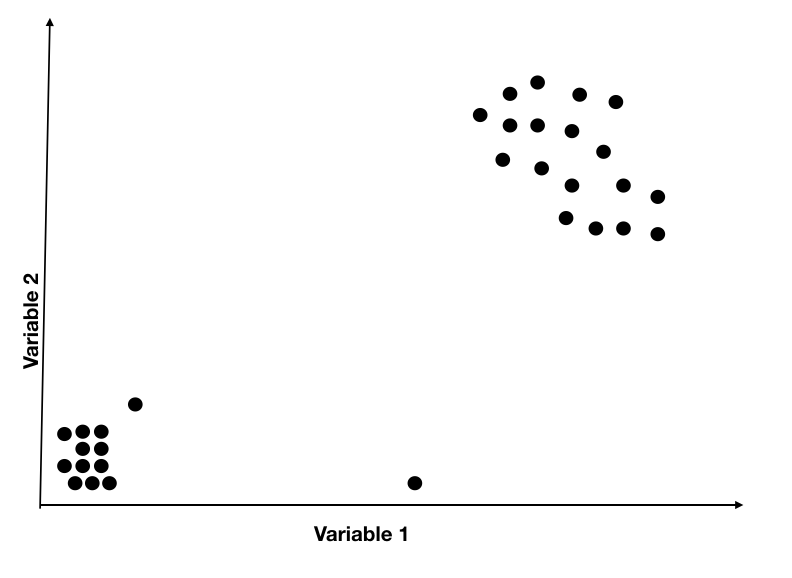
\includegraphics[width=.75\textwidth]{NaiveOutlier}
\end{frame}

\begin{frame}{Why local outliers?}
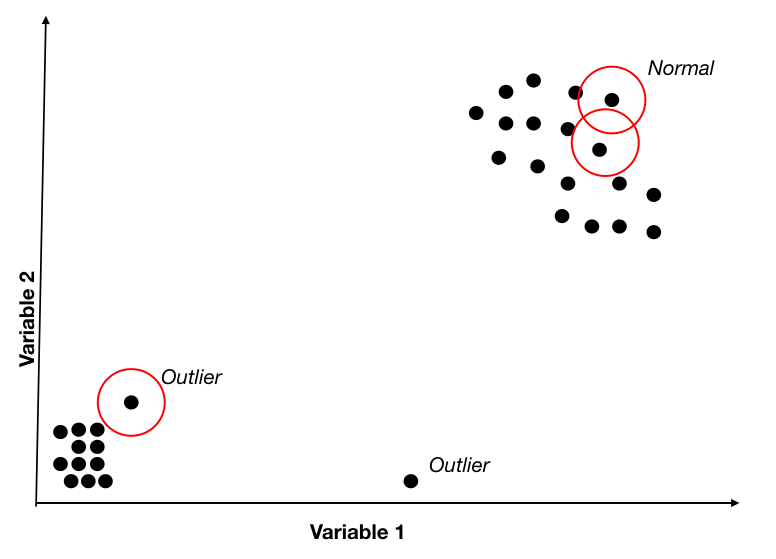
\includegraphics[width=.75\textwidth]{NaiveOutlier2}
\\
\alert{Solutions based on absolute density cannot detect local objetcs}
\end{frame}

\begin{frame}{Local Outlier Factor}
Consider relative density
Let $k$-$\texttt{dist}(\vectorI)$ be the distance of $\vectorI$ to the $k$-th nearest neighbor.
Then the \emph{reachability distance} denoted by $\texttt{reach-dist}$ is
\begin{equation*}
\texttt{reach-dist}(\vectorI,\mathbf{y})=\max(k\texttt{-dist}(\mathbf{y}),\texttt{dist}(\vectorI,\mathbf{y}))
\end{equation*}
Note that $\texttt{reach-dist}$ is not symmetric.
The Local Reachability Density (LRD) is defined by:
\begin{equation*}
\texttt{LRD}_k(\vectorI)=\frac{1}{\frac{\sum_{z \in N_k}\texttt{reach-dist}(\vectorI,\mathbf{z})}{|N_k(\vectorI)|}}
\end{equation*}
which is the inverse of the mean distance of the local reachability of $\vectorI$ and its neighbors.
\end{frame}

\begin{frame}{Local Outlier Factor}
The local outlier factor (LOF) compares the local density with respect to the one from the $k$-nearest neighbors, \emph{i.e.}
\begin{eqnarray*}
\texttt{LOF}_k(\vectorI)&=& \frac{\sum_{z \in N_{k}(\vectorI) \frac{\texttt{lrd}_k(\mathbf{z})}{{\texttt{lrd}_k(\vectorI)}}}}{|N_{k}(\vectorI)|} \\
&=& \frac{\sum_{z \in N_{k}(\vectorI)} \texttt{lrd}_k(\mathbf{z})}{|N_{k}(\vectorI)|\texttt{lrd}_k(\vectorI)}
\end{eqnarray*}
\end{frame}

\begin{frame}{Example Four Points (1/3)}
\begin{center}
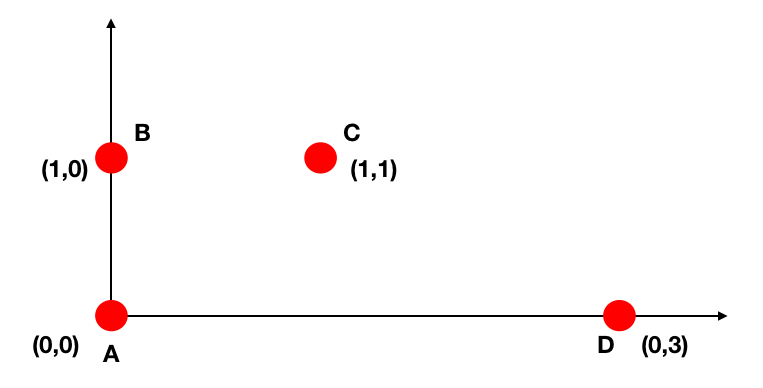
\includegraphics[width=.75\textwidth]{ExampleFourPoints}
\end{center}
\textbf{Example:}
Using the Manhattan distance (a.k.a. taxicab metric or $L_1$ norm, $\forall \mathbf{p},\mathbf{q} \in \mathbb{R}^{d}, \texttt{dist}(\mathbf{p},\mathbf{q})=||\mathbf{p}-\mathbf{q}||_1=\sum_{i=1}^{d}|\mathbf{p}_i-\mathbf{q}_i|$, calcule the local outlier factor, $\texttt{LOF}_k(\vectorI)$ for $k=2$.
\end{frame}

\begin{frame}{Example Four Points (2/3)}
\begin{figure}
\subfigure[$\texttt{dist}(\cdot,\cdot)$]{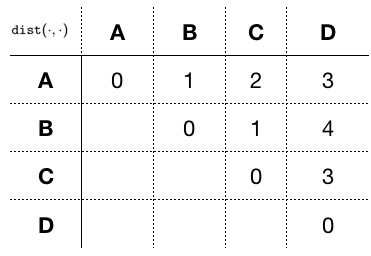
\includegraphics[width=.33\textwidth]{ExampleFourPointsDistance}}
\subfigure[$k\texttt{-dist}(\cdot)$ for $k=1,2,3$]{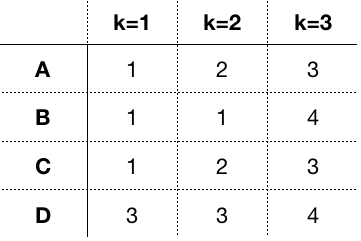
\includegraphics[width=.33\textwidth]{ExampleFourPointsKNNDistance}}\\
\subfigure[Set of $2$-NN, $N_2(\cdot)$]{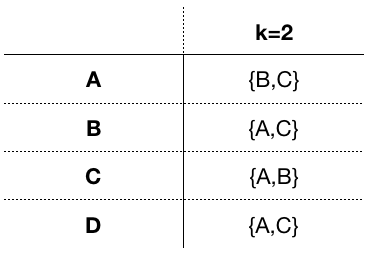
\includegraphics[width=.33\textwidth]{ExampleFourPointsSetKNN}}
\subfigure[2-$\texttt{reach-dist}(\cdot,\cdot)$]{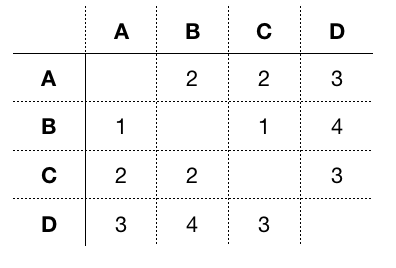
\includegraphics[width=.33\textwidth]{ExampleFourPointsReachScore}}
\end{figure}
\end{frame}

\begin{frame}{Example Four Points (3/3)}
\begin{figure}
\subfigure[$\texttt{LRD}_2(\vectorI)$]{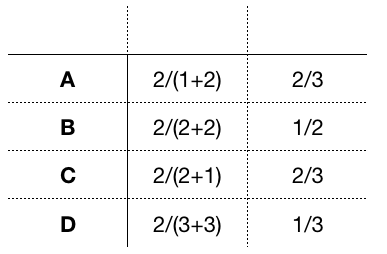
\includegraphics[width=.33\textwidth]{ExampleFourPointsLRD}}
\subfigure[$\texttt{LOF}_2$]{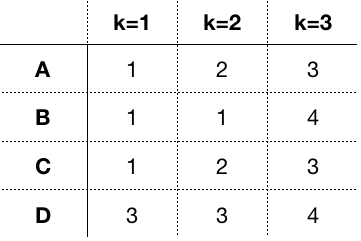
\includegraphics[width=.33\textwidth]{ExampleFourPointsKNNDistance}}\\
\end{figure}
\end{frame}

\begin{frame}
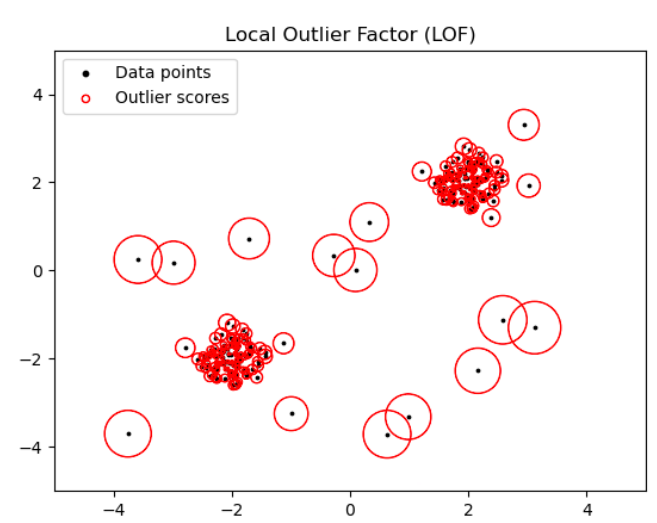
\includegraphics[width=.75\textwidth]{LOFPython}
\end{frame}

\subsection{Evaluating the performance of a score}
\begin{frame}{ROC Curve}
A receiver operating characteristic curve, or \textbf{ROC curve}, is a plot that illustrates the ability of a detector as its discrimination threshold is varied.
The ROC curve is created by plotting the true positive rate (TPR) against the false positive rate (FPR) at various threshold settings
\begin{figure}
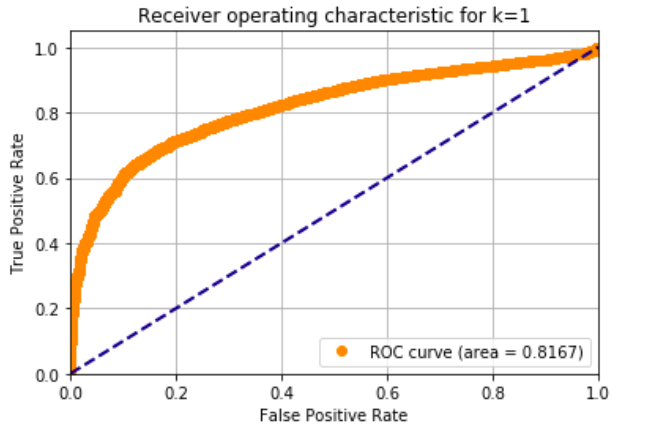
\includegraphics[width=.75\textwidth]{ROC_CURVE}
\end{figure}
\end{frame}

\begin{frame}{Finding the best threshold}
\begin{itemize}
\item The optimal cut off would be where true positive is high and false negative is low
\end{itemize}
\begin{figure}
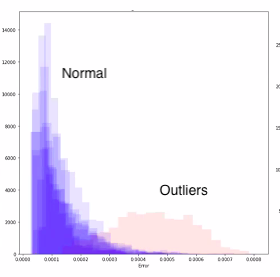
\includegraphics[width=.35\textwidth]{ExampleDetector}
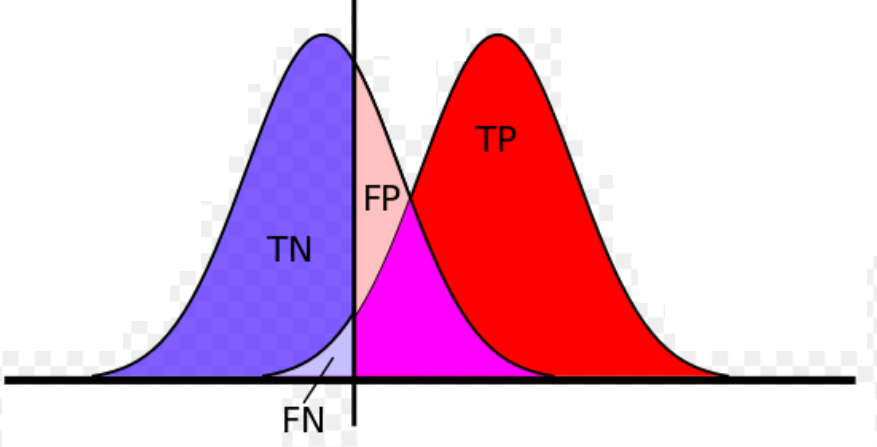
\includegraphics[width=.55\textwidth]{TNFP}
\end{figure}
\end{frame}
%\begin{frame}{Isolation Forest}
%At the basis of the Isolation Forest algorithm there is the tendency of anomalous instances in a dataset to be easier to separate from the rest of the sample (isolate), compared to normal points.
%\end{frame}
\end{document}
